\section{Variable Type Generation Model}
\label{sec:type-gen}

\begin{figure*}[ht]
	\begin{center}
	  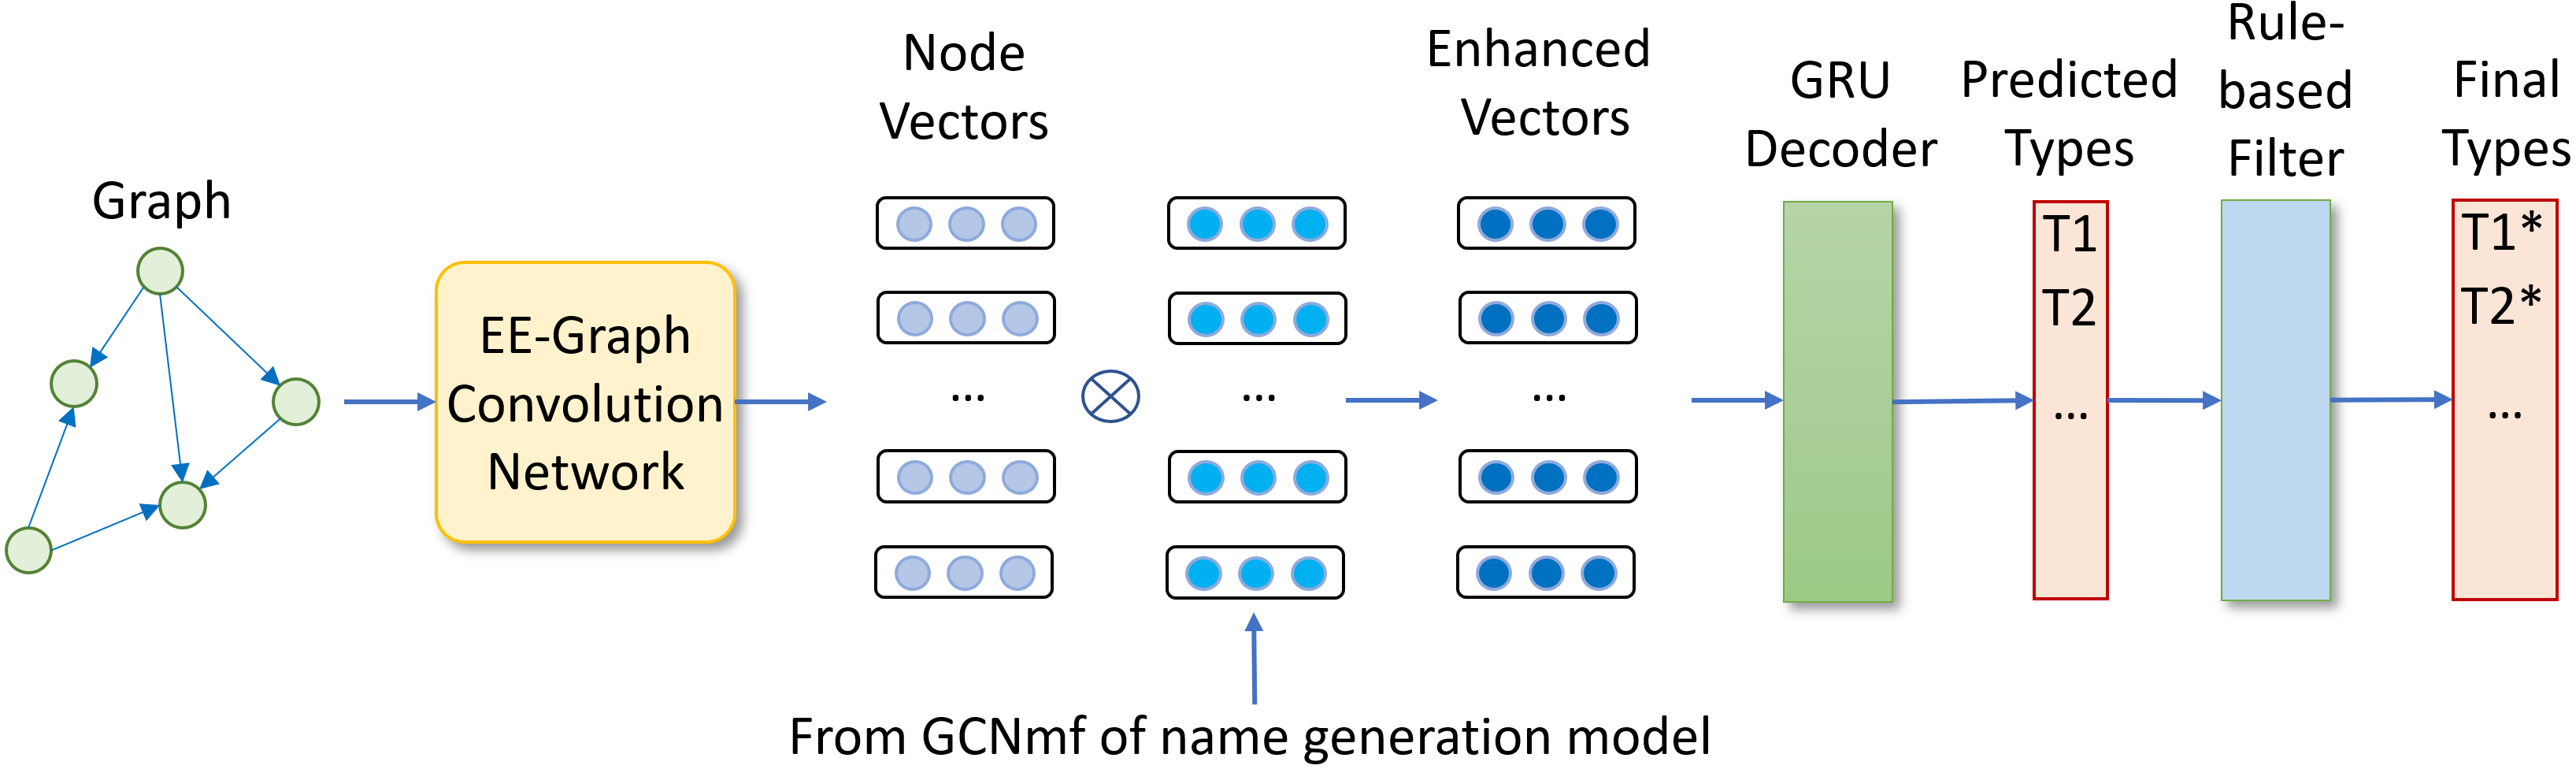
\includegraphics[width=5in]{figures/type-gen-model}
          \vspace{-6pt}
		\caption{The Variable Type Generation Model (VTG)}
		\label{fig:type-gen}
	\end{center}
\end{figure*}

This section presents the Variable Type Generation Model (VTG). During
training, the input is the minified code with all the original
variables’ names and types, and during predicting, it does not have
them. First, we build the TDG and the RG for the given minified code.
The two graphs are combined into a representation graph $G$. For each
node in $G$, we tokenize the names in the corresponding code sequence
of the node. We consider each of them as a sentence and use an
embedding model to build the representation vector for each node in
$G$.

Next, we feed the graph $G$ with those vectors to the
EE-GCN~\cite{ee-gcn}. EE-GCN could accept both node and edge features.
We use the above vectors as node features, and the edge types in the
graph $G$ (built from the TDG and the RG) as the edge features. A key
characteristic of EE-GCN is that it has an edge-aware node update
module and a node-aware edge update module, and two modules works in a
mutual way by updating each other iteratively. Specifically, ``for
each layer, the edge-aware node update module is firstly performed for
aggregating information from neighbors of each node through specific
edges. Then, a node-aware edge update module is used to dynamically
refine the edge representation with its connected node
representations, making the edge representation more informative.''
The output of the EE-GCN model the list of the representation vectors
$V_n$ for all the nodes in the graph $G$.

To further propagate the impact from variable name learning to type
learning, we combine the above vectors $V_n$ with the vectors obtained
from the GCNmf in the Variable Name Generation model. Specifically, we
use the cross-product between the two vectors to produce the final
vectors $V_f$ for the type prediction for all the nodes. Next, we
leverage an Gate Recurrent Unit (GRU) as a decoder, which accepts the
vectors $V_f$s as input and generates the type for the node. (During
training, the type labels are used). Finally, we also apply the
rule-based filter, which performs type-checking to eliminate the
candidates that violate the type inference rules. The final
result include the types for all the nodes including the ones for
variables.

%6> When generating the type, we use some basic rule from parser to
%reduce the possible candidates.

%Variable Type Generation:

%1> Graph edge represent different relations (This may change depends on the graph we finally want to use). Each node is a variable, method call, or a field of an object. We use the name of the variable (minified), method call, or the field as the node feature and use GloVe to learn the representation vector.

%2> We use EGCN that accepts graphs with both node features and edges features as input. Here the edge feature is the edge type. 

%3> The output of EGCN is the generated representation vector $V_r$ for each node. 

%4> We combined the representation vector we get from EGCN with the generated from the next step $V'_r$ (variable name generation) by using the cross-product and get the final generated representation vector for type prediction ($V_f$)

%5> We use a GRU (RNN) as decoder accepts the $V_f$ as input and generates the type for the variables as output.

%6> When generating the type, we use some basic rule from parser to reduce the possible candidates.
